\documentclass[aspectratio=169]{beamer}
\usetheme{Madrid}
\usecolortheme{default}

\usepackage{graphicx}
\usepackage{amsmath}
\usepackage{amsfonts}
\usepackage{listings}
\usepackage{xcolor}
\usepackage{tikz}
\usepackage[utf8]{inputenc}
\usepackage[T1]{fontenc}
\usepackage[hungarian]{babel}

\title{}
\subtitle{Szimbólikus zene generálás - Zha}
\author{Dégi Nándor}
\date{\today}

% Use predefined Python language settings
\lstset{
    language=Python,
    basicstyle=\ttfamily\scriptsize, 
    keywordstyle=\color{blue}\bfseries,
    commentstyle=\color{green!60!black},
    stringstyle=\color{red},
    numbers=left,
    numberstyle=\tiny\color{gray},
    stepnumber=1,
    numbersep=5pt,
    backgroundcolor=\color{gray!10},
    showspaces=false,
    showstringspaces=false,
    showtabs=false,
    frame=single,
    tabsize=2,
    captionpos=b,
    breaklines=true,
    breakatwhitespace=false,
    escapeinside={\%*}{*)},
    aboveskip=3pt,        % Reduced top margin
    belowskip=3pt,        % Reduced bottom margin
    xleftmargin=5pt,      % Reduced left margin
    xrightmargin=5pt,     % Reduced right margin
    framexleftmargin=5pt, % Frame margin
    lineskip=-1pt         % Tighter line spacing
}

\begin{document}

\frame{\titlepage}

\begin{frame}{Áttekintés}
\tableofcontents
\end{frame}

\section{Rendszer Áttekintése}

\begin{frame}{Rendszer Architektúra}
\begin{center}
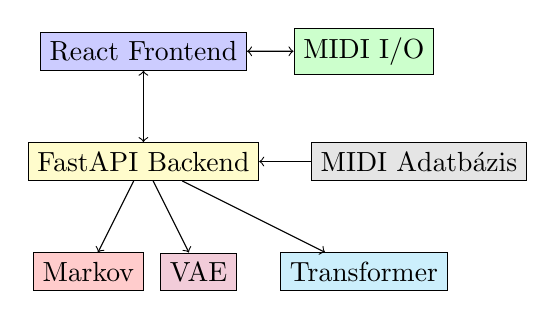
\begin{tikzpicture}[scale=0.7]
    % Frontend
    \node[rectangle, draw, fill=blue!20] (frontend) at (0,4) {React Frontend};
    \node[rectangle, draw, fill=green!20] (midi) at (4,4) {MIDI I/O};
    
    % Backend API
    \node[rectangle, draw, fill=yellow!20] (api) at (0,2) {FastAPI Backend};
    
    % Models
    \node[rectangle, draw, fill=red!20] (markov) at (-1,0) {Markov};
    \node[rectangle, draw, fill=purple!20] (vae) at (1,0) {VAE};
    \node[rectangle, draw, fill=cyan!20] (transformer) at (4,0) {Transformer};
    
    % Data
    \node[rectangle, draw, fill=gray!20] (data) at (5,2) {MIDI Adatbázis};
    
    % Arrows
    \draw[<->] (frontend) -- (api);
    \draw[<->] (frontend) -- (midi);
    \draw[->] (api) -- (markov);
    \draw[->] (api) -- (vae);
    \draw[->] (api) -- (transformer);
    \draw[->] (data) -- (api);
\end{tikzpicture}
\end{center}
\end{frame}

\section{MIDI Adatfeldolgozás}

\begin{frame}[fragile]{MIDI Adattranszformációs Pipeline}
\textbf{Alapvető Adatfeldolgozási Funkciók:}

\begin{lstlisting}
def parse_midi(midi_path):
    midi_data = pretty_midi.PrettyMIDI(midi_path)
    feature = np.zeros(128, dtype=np.float32)
    
    for instrument in midi_data.instruments:
        for note in instrument.notes:
            feature[note.pitch] += note.velocity / 127.0
    
    if np.sum(feature) > 0:
        feature = feature / np.sum(feature)
    
    return feature
\end{lstlisting}

\textbf{Kulcs Transzformációk:}
\begin{itemize}
    \item Hangmagasság információ kinyerése minden hangszerből
    \item Hangerő súlyozás (0-1 normalizált)
    \item Valószínűségi eloszlás létrehozása 128 MIDI hangjegyre
    \item Normalizálás 1.0 összegre
\end{itemize}
\end{frame}

\section{Markov-lánc Modell}

\begin{frame}[fragile]{Markov-lánc Modell Architektúra}
\begin{center}
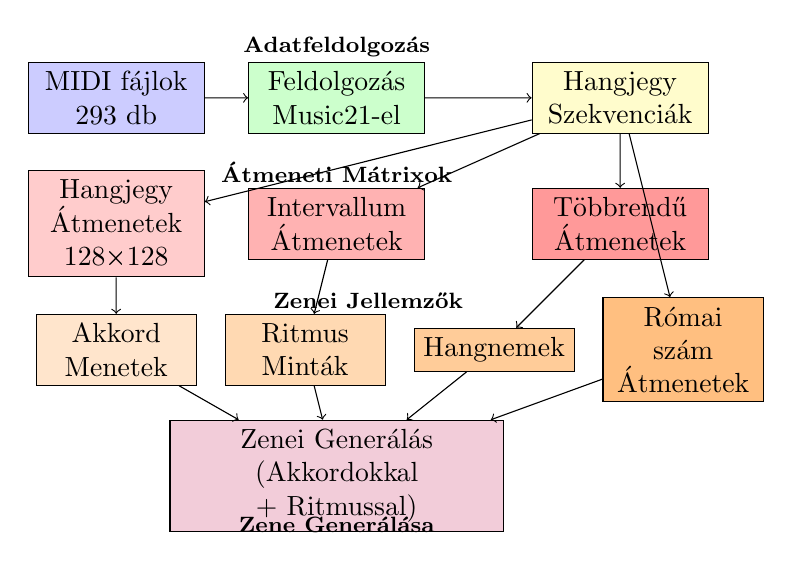
\begin{tikzpicture}[scale=0.8]
    % Input processing
    \node[rectangle, draw, fill=blue!20, text width=2cm, align=center] (midi_files) at (-1,6) {MIDI fájlok\\293 db};
    \node[rectangle, draw, fill=green!20, text width=2cm, align=center] (music21) at (2.5,6) {Feldolgozás\\Music21-el};
    \node[rectangle, draw, fill=yellow!20, text width=2cm, align=center] (sequences) at (7,6) {Hangjegy\\Szekvenciák};

    % Transition matrices
    \node[rectangle, draw, fill=red!20, text width=2cm, align=center] (note_trans) at (-1,4) {Hangjegy\\Átmenetek\\128×128};
    \node[rectangle, draw, fill=red!30, text width=2cm, align=center] (interval_trans) at (2.5,4) {Intervallum\\Átmenetek};
    \node[rectangle, draw, fill=red!40, text width=2cm, align=center] (multi_order) at (7,4) {Többrendű\\Átmenetek};

    % Musical features
    \node[rectangle, draw, fill=orange!20, text width=1.8cm, align=center] (chord_prog) at (-1,2) {Akkord\\Menetek};
    \node[rectangle, draw, fill=orange!30, text width=1.8cm, align=center] (rhythm) at (2,2) {Ritmus\\Minták};
    \node[rectangle, draw, fill=orange!40, text width=1.8cm, align=center] (keys) at (5,2) {Hangnemek};
    \node[rectangle, draw, fill=orange!50, text width=1.8cm, align=center] (roman) at (8,2) {Római szám\\Átmenetek};

    % Generation
    \node[rectangle, draw, fill=purple!20, text width=4cm, align=center] (generation) at (2.5,0) {Zenei Generálás\\(Akkordokkal + Ritmussal)};

    % Arrows
    \draw[->] (midi_files) -- (music21);
    \draw[->] (music21) -- (sequences);
    \draw[->] (sequences) -- (note_trans);
    \draw[->] (sequences) -- (interval_trans);
    \draw[->] (sequences) -- (multi_order);
    \draw[->] (note_trans) -- (chord_prog);
    \draw[->] (interval_trans) -- (rhythm);
    \draw[->] (multi_order) -- (keys);
    \draw[->] (sequences) -- (roman);
    \draw[->] (chord_prog) -- (generation);
    \draw[->] (rhythm) -- (generation);
    \draw[->] (keys) -- (generation);
    \draw[->] (roman) -- (generation);

    % Layer labels
    \node[above, font=\footnotesize\bfseries] at (2.5,6.5) {Adatfeldolgozás};
    \node[above, font=\footnotesize\bfseries] at (2.5,4.5) {Átmeneti Mátrixok};
    \node[above, font=\footnotesize\bfseries] at (3,2.5) {Zenei Jellemzők};
    \node[below, font=\footnotesize\bfseries] at (2.5,-0.5) {Zene Generálása};
\end{tikzpicture}
\end{center}
\end{frame}

\begin{frame}[fragile]{Markov Modell Implementáció}
\textbf{Alapvető felépítés:}

\begin{lstlisting}
class MarkovChain:
    def __init__(self, order=2, max_interval=12):
        self.transitions = np.zeros((128, 128), dtype=np.float32)
        self.interval_transitions = {}
        
        self.musical_features = {
            'chord_progressions': {},
            'rhythm_patterns': {},
            'roman_numeral_transitions': {},
            'common_keys': {}
        }
\end{lstlisting}

\textbf{Kulcs komponensek:}
\begin{itemize}
    \item \textbf{128×128 átmeneti mátrix}: P(hangjegy\_j | hangjegy\_i)
    \item \textbf{Intervallum átmenetek}: Relatív hangmagasság változások
    \item \textbf{Többrendű kontextus}: Előző 2-3 hangjegy alapján
\end{itemize}
\end{frame}

\begin{frame}[fragile]{Átmeneti Mátrix Példa}
\textbf{Egyszerűsített átmeneti mátrix (C-dúr részlet):}

\vspace{0.5cm}

\begin{center}
\begin{tabular}{c|cccccc}
\textbf{Hangjegy} & \textbf{C4} & \textbf{D4} & \textbf{E4} & \textbf{F4} & \textbf{G4} & \textbf{...} \\
\hline
\textbf{C4 (60)} & 0.15 & 0.25 & 0.20 & 0.10 & 0.20 & ... \\
\textbf{D4 (62)} & 0.20 & 0.10 & 0.25 & 0.15 & 0.15 & ... \\
\textbf{E4 (64)} & 0.30 & 0.20 & 0.05 & 0.25 & 0.10 & ... \\
\textbf{F4 (65)} & 0.15 & 0.10 & 0.20 & 0.15 & 0.25 & ... \\
\textbf{G4 (67)} & 0.35 & 0.15 & 0.10 & 0.20 & 0.10 & ... \\
\end{tabular}
\end{center}

\vspace{0.3cm}

\textit{Minden sor összege = 1.0. Mátrix[i,j] = P(következő hangjegy = j | jelenlegi = i)}

\textbf{Intervallum átmenetek:}
\begin{itemize}
    \item \textbf{+2 félhang}: Nagy szekund felfelé (C→D)
    \item \textbf{-5 félhang}: Kvart lefelé (G→D)
    \item \textbf{0 félhang}: Ismétlés
\end{itemize}
\end{frame}

\begin{frame}[fragile]{Markov Tanítási Folyamat}

\begin{lstlisting}
def train_markov_model(midi_dir="dataset/midi", order=2):
    model = MarkovChain(order=order)
    
    with multiprocessing.Pool() as pool:
        scores = list(tqdm(
            pool.imap(process_midi_file, midi_files),
            total=len(midi_files)
        ))
    
    note_sequences = []
    for score in scores:
        sequence = extract_note_sequence_from_score(score)
        note_sequences.append(sequence)
    
    model.train(note_sequences)
    model.save("trained_markov.npy")
\end{lstlisting}
\end{frame}

\begin{frame}[fragile]{Zenei Jellemzők Kinyerése}
\textbf{Mit tanul meg a modell:}

\begin{lstlisting}
def extract_musical_features(self, midi_sequences):
    features = {
        'chord_progressions': [],  # I-V-vi-IV
        'rhythm_patterns': [],     # Ütemenkénti ritmusok
        'roman_numeral_transitions': {},  # I→V, V→vi
        'common_keys': {},         # C major, A minor
        'time_signatures': {}      # 4/4, 3/4
    }
    
    # Music21 segítségével zenei analízis
    for stream in all_streams:
        key_analysis = stream.analyze('key')
        chords = stream.chordify()
\end{lstlisting}

\begin{itemize}
    \item \textbf{Akkordmenetek}: I-V-vi-IV, ii-V-I típusú progressziók
    \item \textbf{Ritmus minták}: Ütemenkénti hangjegy eloszlások
    \item \textbf{Hangnem kapcsolatok}: Gyakori modulációk
\end{itemize}
\end{frame}

\begin{frame}[fragile]{Generálási Módszerek}
\textbf{Többféle generálási megközelítés:}

\begin{lstlisting}
def generate_sequence(self, start_note=60, length=32):
    sequence = [start_note]
    current_note = start_note
    
    for _ in range(length - 1):
        probs = self.transitions[current_note]
        next_note = np.random.choice(128, p=probs)
        sequence.append(next_note)
        current_note = next_note
    
    return sequence

def generate_with_chords(self, key_context="C major"):
    chords = self.generate_chord_progression(key_context)
    melody = self.generate_sequence_for_chords(chords)
    return {'notes': melody, 'chords': chords}
\end{lstlisting}
\end{frame}

\begin{frame}[fragile]{Expresszi kiszámi generálás}
\textbf{Komplex zenei elemek kombinálása:}

\begin{lstlisting}
def generate_expressive_sequence(self, key_context, complexity=0.7):
    if complexity < 0.3:
        time_sig = "4/4"
    else:
        time_sig = random.choice(["4/4", "3/4", "6/8"])
    
    chords = self.generate_chord_progression(key_context)
    
    rhythmic_seq = self.generate_rhythmic_sequence(
        key_context=key_context,
        time_signature=time_sig
    )
    
    return {'notes': notes, 'chords': chords, 'rhythm': rhythms}
\end{lstlisting}

\textbf{Előnyök:}
\begin{itemize}
    \item Gyors tanítás (5 perc 293 MIDI fájlból)
    \item Zeneileg értelmes kimenet
    \item Valós időben generálás
\end{itemize}
\end{frame}

\section{VAE Modell}

\begin{frame}[fragile]{VAE Modell Részletes Architektúra}
\begin{center}
\resizebox{0.95\linewidth}{!}{%
\begin{tikzpicture}{scale}
    % Input
    \node[rectangle, draw, fill=blue!20, text width=1.5cm, align=center] (input) at (0,6) {MIDI\\128 dim};
    
    % Encoder pathway
    \node[rectangle, draw, fill=green!20, text width=1.5cm, align=center] (enc_linear1) at (2,6) {Linear\\128→512};
    \node[rectangle, draw, fill=green!30, text width=1.5cm, align=center] (enc_norm1) at (4,6) {LayerNorm\\512};
    \node[rectangle, draw, fill=green!40, text width=1.5cm, align=center] (enc_res1) at (6,6) {ResBlock\\512};
    
    \node[rectangle, draw, fill=green!20, text width=1.5cm, align=center] (enc_linear2) at (2,4) {Linear\\512→256};
    \node[rectangle, draw, fill=green!30, text width=1.5cm, align=center] (enc_norm2) at (4,4) {LayerNorm\\256};
    \node[rectangle, draw, fill=green!40, text width=1.5cm, align=center] (enc_res2) at (6,4) {ResBlock\\256};
    
    \node[rectangle, draw, fill=red!20, text width=1.5cm, align=center] (enc_output) at (8,5) {Linear\\256→256};
    
    % Latent space
    \node[rectangle, draw, fill=red!40, text width=1cm, align=center] (mu) at (10,6) {μ\\128};
    \node[rectangle, draw, fill=red!40, text width=1cm, align=center] (logvar) at (10,4) {log σ²\\128};
    \node[rectangle, draw, fill=yellow!20, text width=1.5cm, align=center] (reparam) at (12,5) {Reparam\\Trick};
    \node[rectangle, draw, fill=orange!20, text width=1cm, align=center] (z) at (14,5) {z\\128};
    
    % Decoder pathway
    \node[rectangle, draw, fill=purple!20, text width=1.5cm, align=center] (dec_linear1) at (2,2) {Linear\\128→256};
    \node[rectangle, draw, fill=purple!30, text width=1.5cm, align=center] (dec_norm1) at (4,2) {LayerNorm\\256};
    \node[rectangle, draw, fill=purple!40, text width=1.5cm, align=center] (dec_res1) at (6,2) {ResBlock\\256};
    
    \node[rectangle, draw, fill=purple!20, text width=1.5cm, align=center] (dec_linear2) at (2,0) {Linear\\256→512};
    \node[rectangle, draw, fill=purple!30, text width=1.5cm, align=center] (dec_norm2) at (4,0) {LayerNorm\\512};
    \node[rectangle, draw, fill=purple!40, text width=1.5cm, align=center] (dec_res2) at (6,0) {ResBlock\\512};
    
    \node[rectangle, draw, fill=blue!20, text width=1.5cm, align=center] (output) at (8,1) {Linear\\512→128};
    \node[rectangle, draw, fill=blue!40, text width=1.5cm, align=center] (sigmoid) at (10,1) {Sigmoid\\128};
    
    % Arrows
    \draw[->] (input) -- (enc_linear1);
    \draw[->] (enc_linear1) -- (enc_norm1);
    \draw[->] (enc_norm1) -- (enc_res1);
    \draw[->] (enc_res1) -- (enc_linear2);
    \draw[->] (enc_linear2) -- (enc_norm2);
    \draw[->] (enc_norm2) -- (enc_res2);
    \draw[->] (enc_res2) -- (enc_output);
    \draw[->] (enc_output) -- (mu);
    \draw[->] (enc_output) -- (logvar);
    \draw[->] (mu) -- (reparam);
    \draw[->] (logvar) -- (reparam);
    \draw[->] (reparam) -- (z);
    
    \draw[->] (z) -- (dec_linear1);
    \draw[->] (dec_linear1) -- (dec_norm1);
    \draw[->] (dec_norm1) -- (dec_res1);
    \draw[->] (dec_res1) -- (dec_linear2);
    \draw[->] (dec_linear2) -- (dec_norm2);
    \draw[->] (dec_norm2) -- (dec_res2);
    \draw[->] (dec_res2) -- (output);
    \draw[->] (output) -- (sigmoid);
    
    % Labels
    \node[above] at (4,6.5) {\textbf{Encoder}};
    \node[above] at (12,6.5) {\textbf{Látens Tér}};
    \node[above] at (4,2.5) {\textbf{Decoder}};
\end{tikzpicture}%
}
\end{center}
\end{frame}


\begin{frame}[fragile]
\textbf{Pytorch-ban:}
\begin{lstlisting}
class VAEModel(nn.Module):
    def __init__(self, input_dim=128, latent_dim=128, beta=1.0):
        self.encoder_input = nn.Linear(input_dim, 512)
        self.encoder_res1 = ResidualBlock(512)
        self.encoder_hidden = nn.Linear(512, 256)
        self.encoder_res2 = ResidualBlock(256)
        self.encoder_output = nn.Linear(256, latent_dim * 2)
        
        self.decoder_input = nn.Linear(latent_dim, 256)
        self.decoder_res1 = ResidualBlock(256)
        self.decoder_hidden = nn.Linear(256, 512)
        self.decoder_res2 = ResidualBlock(512)
        self.decoder_output = nn.Linear(512, input_dim)
        
        self.beta = beta
\end{lstlisting}

\textbf{Kulcs Jellemzők:}
\begin{itemize}
    \item Reziduális blokkok stabil tanításhoz
    \item Réteg normalizáció jobb konvergenciáért
    \item Beta paraméter kontrollált látens térhez
    \item SiLU aktivációs funkciók
\end{itemize}
\end{frame}

\begin{frame}[fragile]{VAE Tanítási Implementáció}

    \begin{lstlisting}
    def train_epoch(model, dataloader, optimizer, scaler, consistency_weight=0.1):
        for batch in dataloader:
            with autocast(device_type='cuda'):
                recon_batch, mu, logvar = model(batch)
            
            # Hagyományos VAE veszteségek
            recon_loss = F.binary_cross_entropy(recon_batch, batch, reduction='sum')
            kl_loss = -0.5 * torch.sum(1 + logvar - mu.pow(2) - logvar.exp())
            
            # Konzisztencia veszteség zenei simításért
            note_diffs = torch.abs(recon_batch[:, 1:] - recon_batch[:, :-1])
            consistency_loss = torch.mean(note_diffs) * consistency_weight
            
            # Teljes veszteség beta-VAE módszerrel
            loss = recon_loss + model.beta * kl_loss + consistency_loss
            
            # Gradiens akkumuláció kevert precizitással
            scaler.scale(loss / accumulation_steps).backward()
            if (i + 1) % accumulation_steps == 0:
                scaler.step(optimizer)
                scaler.update()
    \end{lstlisting}
    
    \textbf{Tanítási Optimalizációk:}
    \begin{itemize}
        \item \textbf{Beta-VAE}: Kontrollált látens tér (beta=0.5)
        \item \textbf{Konzisztencia veszteség}: Simább zenei átmenetek
        \item \textbf{LRU cache}: Hatékony MIDI betöltés (500 fájl cache)
        \item \textbf{Kevert precizitás}: GPU memória optimalizáció
        \item \textbf{Gradiens akkumuláció}: Nagyobb batch méret szimuláció
    \end{itemize}
    \end{frame}

\begin{frame}[fragile]{VAE Generálási Képességek}

\begin{lstlisting}
def sample(self, num_samples=1, temperature=0.8, device='cuda'):
    with torch.no_grad():
        z = torch.randn(num_samples, self.latent_dim, device=device) * temperature
        return self.decode(z)

def interpolate(self, x1, x2, steps=10):
    with torch.no_grad():
        mu1, _ = torch.chunk(self.encode(x1), 2, dim=-1)
        mu2, _ = torch.chunk(self.encode(x2), 2, dim=-1)
        
        alphas = torch.linspace(0, 1, steps)
        z_interp = torch.stack([(1-a)*mu1 + a*mu2 for a in alphas])
        
        return self.decode(z_interp)
\end{lstlisting}

\textbf{Generálási Funkciók:}
\begin{itemize}
    \item Hőmérséklet-vezérelt mintavételezés
    \item Sima interpoláció darabok között
    \item Látens tér felfedezés
    \item ONNX export telepítéshez
\end{itemize}
\end{frame}

\section{Transformer Modell}

\begin{frame}[fragile]{Transformer Modell Architektúra}
\begin{center}
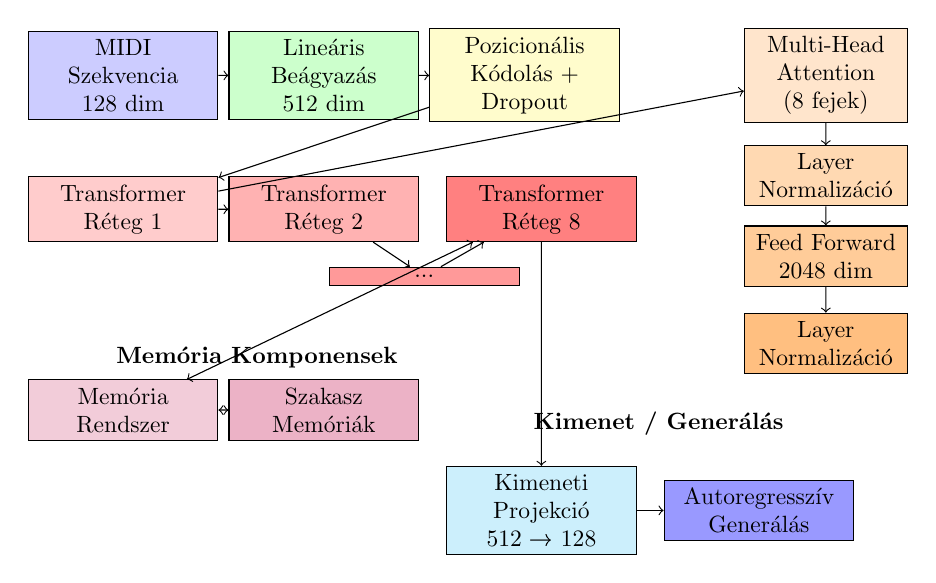
\begin{tikzpicture}[scale=0.85, every node/.style={transform shape}]
    % === Input Processing ===
    \node[rectangle, draw, fill=blue!20, text width=2.6cm, align=center] (input) at (0,6.5) {MIDI\\Szekvencia\\128 dim};
    \node[rectangle, draw, fill=green!20, text width=2.6cm, align=center] (embedding) at (3,6.5) {Lineáris\\Beágyazás\\512 dim};
    \node[rectangle, draw, fill=yellow!20, text width=2.6cm, align=center] (posenc) at (6,6.5) {Pozicionális\\Kódolás +\\Dropout};

    % === Transformer Stack ===
    \node[rectangle, draw, fill=red!20, text width=2.6cm, align=center] (trans1) at (0,4.5) {Transformer\\Réteg 1};
    \node[rectangle, draw, fill=red!30, text width=2.6cm, align=center] (trans2) at (3,4.5) {Transformer\\Réteg 2};
    \node[rectangle, draw, fill=red!40, text width=2.6cm, align=center] (trans3) at (4.5,3.5) {...};
    \node[rectangle, draw, fill=red!50, text width=2.6cm, align=center] (trans8) at (6.25,4.5) {Transformer\\Réteg 8};

    % === Transformer Details ===
    \node[rectangle, draw, fill=orange!20, text width=2.2cm, align=center] (mha) at (10.5,6.5) {Multi-Head\\Attention\\(8 fejek)};
    \node[rectangle, draw, fill=orange!30, text width=2.2cm, align=center] (norm1) at (10.5,5) {Layer\\Normalizáció};
    \node[rectangle, draw, fill=orange!40, text width=2.2cm, align=center] (ffn) at (10.5,3.8) {Feed Forward\\2048 dim};
    \node[rectangle, draw, fill=orange!50, text width=2.2cm, align=center] (norm2) at (10.5,2.5) {Layer\\Normalizáció};

    % === Memory System ===
    \node[rectangle, draw, fill=purple!20, text width=2.6cm, align=center] (mem) at (0,1.5) {Memória\\Rendszer};
    \node[rectangle, draw, fill=purple!30, text width=2.6cm, align=center] (sectmem) at (3,1.5) {Szakasz\\Memóriák};

    % === Output ===
    \node[rectangle, draw, fill=cyan!20, text width=2.6cm, align=center] (proj) at (6.25,0) {Kimeneti\\Projekció\\512 → 128};
    \node[rectangle, draw, fill=blue!40, text width=2.6cm, align=center] (gen) at (9.5,0) {Autoregresszív\\Generálás};

    % === Arrows ===
    \draw[->] (input) -- (embedding);
    \draw[->] (embedding) -- (posenc);
    \draw[->] (posenc) -- (trans1);
    \draw[->] (trans1) -- (trans2);
    \draw[->] (trans2) -- (trans3);
    \draw[->] (trans3) -- (trans8);
    
    \draw[->] (trans1) -- (mha);
    \draw[->] (mha) -- (norm1);
    \draw[->] (norm1) -- (ffn);
    \draw[->] (ffn) -- (norm2);

    \draw[<->] (trans8) -- (mem);
    \draw[<->] (mem) -- (sectmem);

    \draw[->] (trans8) -- (proj);
    \draw[->] (proj) -- (gen);

    % === Section Labels ===
    \node[above] at (2,2) {\textbf{Memória Komponensek}};
    \node[above] at (8,1) {\textbf{Kimenet / Generálás}};
\end{tikzpicture}
\end{center}
\end{frame}


\begin{frame}[fragile]{A Transformer Osztály}
\textbf{Egyedi memória architektúra strukturált generáláshoz:}

\begin{lstlisting}
class TransformerModel(nn.Module):
    def __init__(self, input_dim=128, embed_dim=512, num_heads=8, num_layers=8):
        self.embedding = nn.Linear(input_dim, embed_dim)
        self.pos_encoder = PositionalEncoding(embed_dim)
        
        encoder_layers = nn.TransformerEncoderLayer(
            d_model=embed_dim, nhead=num_heads,
            dim_feedforward=2048, dropout=0.1,
            batch_first=True
        )
        self.transformer_encoder = nn.TransformerEncoder(
            encoder_layers, num_layers=num_layers
        )
        
        self.output_projection = nn.Linear(embed_dim, input_dim)
        
        self.memory = None
        self.section_memories = {}
\end{lstlisting}
\end{frame}

\begin{frame}[fragile]{Hol generál?}
    \begin{lstlisting}
    def generate_with_structure(self, seed, num_sections=4, section_length=16):
        self.reset_memory()
        all_outputs = []
        
        for section_id in range(num_sections):
            if section_id in self.section_memories:
                self.memory = self.section_memories[section_id]
            
            section_output = self._generate_section(
                seed, steps=section_length, temperature=0.8
            )
            
            self.section_memories[section_id] = self.memory
            all_outputs.append(section_output)
        
        return torch.cat(all_outputs, dim=1)
    \end{lstlisting}
\end{frame}

\begin{frame}[fragile]{Transformer Tanítási Stratégia}

\begin{lstlisting}
def train_transformer_model(epochs=100, batch_size=64):
    model = TransformerModel().to(device)
    
    optimizer = torch.optim.AdamW(model.parameters(), lr=1e-4, weight_decay=1e-4)
    scheduler = torch.optim.lr_scheduler.OneCycleLR(
        optimizer, max_lr=1e-4,
        total_steps=epochs * len(dataloader),
        pct_start=0.1, anneal_strategy='cos'
    )
    
    scaler = torch.amp.GradScaler()
    
    for epoch in range(epochs):
        for batch in dataloader:
            with autocast(device_type='cuda'):
                output = model(batch)
                loss = F.mse_loss(output, batch)
            
            scaler.scale(loss).backward()
            scaler.step(optimizer)
            scaler.update()
            scheduler.step()
    
    torch.jit.script(model.cpu()).save("trained_transformer_jit.pt")
\end{lstlisting}
\end{frame}

\begin{frame}[fragile]{Transformer Generálási Funkciók}
\textbf{Speciális generálási képességek:}

\begin{lstlisting}
def generate_with_structure(self, seed, num_sections=4, section_length=16):
    self.reset_memory()
    all_outputs = []
    
    for section_id in range(num_sections):
        if section_id in self.section_memories:
            self.memory = self.section_memories[section_id]
        
        section_output = self._generate_section(
            seed, steps=section_length, temperature=0.8
        )
        
        self.section_memories[section_id] = self.memory
        all_outputs.append(section_output)
    
    return torch.cat(all_outputs, dim=1)
\end{lstlisting}
\end{frame}

\section{Metrikák}

\begin{frame}{Modell Metrikák}
    \begin{center}
    \textbf{Tanítási Teljesítmény - 293 MIDI Dal Alapján}
    
    \vspace{0.5cm}
    
    \begin{tabular}{|l|c|c|c|c|}
    \hline
    \textbf{Modell} & \textbf{Tanítási Idő} \\
    \hline
    \textbf{Markov-lánc} & \textcolor{black}{\textbf{5 perc}} \\
    \hline
    \textbf{VAE} & \textcolor{black}{55 perc} \\
    \hline
    \textbf{Transformer} & \textcolor{black}{1ó 5p} \\
    \hline
    \end{tabular}
    
    \vspace{0.5cm}
    
    \textbf{Paraméterek és hardware:}
    \begin{itemize}
        \item \textbf{Adathalmaz}: 293 MIDI fájl (7.5 MB)
        \item \textbf{Hardware}: NVIDIA RTX 4050, 6GB RAM
        \item \textbf{Batch méret}: Markov (-), VAE (128), Transformer (64)
        \item \textbf{Epoch számok}: Markov (1 iteráció), VAE (100), Transformer (100)
    \end{itemize}
    
    \vspace{0.3cm}
    
    \begin{center}
    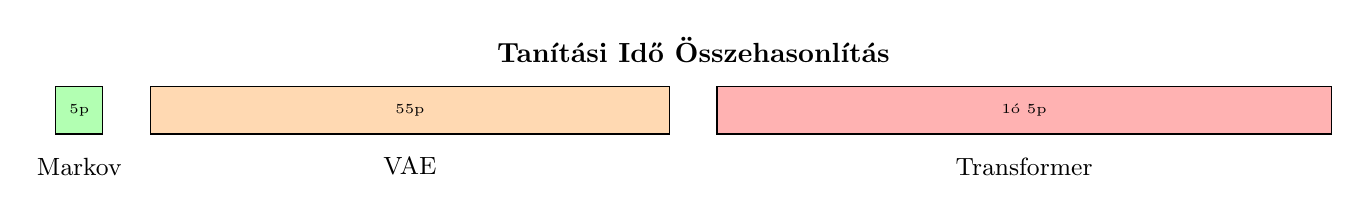
\begin{tikzpicture}[scale=0.6]
        % Training time bar chart
        \draw[fill=green!30] (0,0) rectangle (1,1) node[midway] {\tiny 5p};
        \draw[fill=orange!30] (2,0) rectangle (13,1) node[midway] {\tiny 55p};
        \draw[fill=red!30] (14,0) rectangle (27,1) node[midway] {\tiny 1ó 5p};
        
        \node[below] at (0.5,-0.3) {\small Markov};
        \node[below] at (7.5,-0.3) {\small VAE};
        \node[below] at (20.5,-0.3) {\small Transformer};
        
        \node[above] at (13.5,1.3) {\textbf{Tanítási Idő Összehasonlítás}};
    \end{tikzpicture}
    \end{center}
    \end{center}
    \end{frame}

\begin{frame}
\vspace{1cm}
\begin{center}
\textbf{Köszi a figyelmet!}
\textbf{:)}

\end{center}
\end{frame}

\end{document}